\chapter{Diseño de algoritmo}
\section{Introducción}
En este capítulo se pretende abordar el diseño para llevar a cabo el objetivo principal y algunos de los específicos del proyecto.

\section{Diseño general de trabajo}
En la figura \ref{fig:esquema} se observan las partes que componen el trabajo del sistema. En este sentido, es necesario hacer una diferenciación entre la parte \textit{offline} y la parte \textit{online} ya que cada parte por separado conlleva tareas específicas.

\begin{figure}[h!]
    \centering
    \begin{subfigure}[b]{0.7\textwidth}
        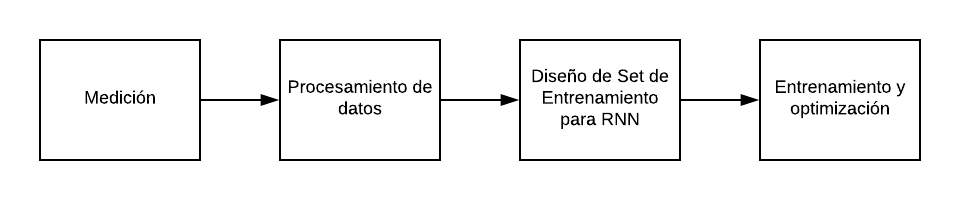
\includegraphics[width=\textwidth]{./images/online}
        \caption{Etapa Online}
        \label{fig:Online}
    \end{subfigure}
    
    \begin{subfigure}[b]{0.4\textwidth}
        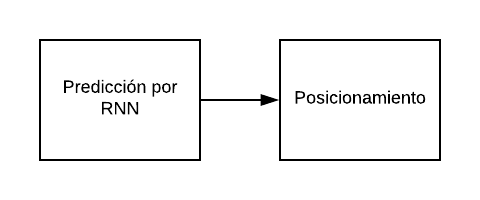
\includegraphics[width=\textwidth]{./images/offline}
        \caption{Etapa Offline}
        \label{fig:offline}
    \end{subfigure}
    \caption{Diagrama General de operación de Algoritmo de posicionamiento}
    \label{fig:esquema}
\end{figure}

\subsection{Offline}
\subsubsection{Medición}

En éste módulo se extraerán los datos a partir de un ordenador de placa reducida, Raspberry Pi 2. Esta tendrá por función medir los niveles de intensidad de potencia de cada uno de los Access Points dispuestos en el pasillo de segundo piso.

\subsubsection{Extracción y procesamiento de datos}
En esta módulo lo que se llevará a cabo es procesar los datos a fin de que la información entregada por la tarjeta permita identificar claramente la MAC del AP, el \ac{ESSID} para construir el dataset de entrenamiento.

\subsubsection{Diseño de Set de Entrenamiento}

El objetivo de este módulo es el de limpiar el dataset de entrenamiento, es decir, remover datos que no aporten a la medición, a la vez que se construye el archivo CSV que contiene las potencias y las direcciones MAC, junto con el ESSID.

\subsubsection{Entrenamiento y Optimización}
En esta parte se construirá la RNN que usará los datos que se recolectaron anteriormente para entrenar la RNN, ajustar los pesos y realizar los test que permitan obtener una mejor precisión en el posicionamiento.

\subsection{Online}

\subsubsection{Predicción por RNN}
En este módulo se hará la identificación de los niveles de potencia recibidos de los AP's por el dispositivo a posicionar.
Luego, estos se comunicarán con la placa Raspberry Pi para entregar un vector con las potencias, las cuales se probarán en la red, entregando la respuesta en forma de coordenadas de la ubicación del dispositivo.

\subsubsection{Posicionamiento}
En esta parte se desarrollará una interfaz que permita visualizar la posición del usuario respecto del mapa del segundo piso. En ella se podrá ver cómo el usuario se desplaza y cerca de qué AP's se encuentra.

